% Use only LaTeX2e, calling the article.cls class and 12-point type.

\documentclass[12pt]{article}

% Users of the {thebibliography} environment or BibTeX should use the
% scicite.sty package, downloadable from *Science* at
% www.sciencemag.org/about/authors/prep/TeX_help/ .
% This package should properly format in-text
% reference calls and reference-list numbers.

\usepackage{scicite}

\usepackage{graphicx}
\usepackage{fancyvrb}

% Use times if you have the font installed; otherwise, comment out the
% following line.

\usepackage{times}
\usepackage{hyperref}
\usepackage{float}

% The preamble here sets up a lot of new/revised commands and
% environments.  It's annoying, but please do *not* try to strip these
% out into a separate .sty file (which could lead to the loss of some
% information when we convert the file to other formats).  Instead, keep
% them in the preamble of your main LaTeX source file.


% The following parameters seem to provide a reasonable page setup.

\topmargin 0.0cm
\oddsidemargin 0.2cm
\textwidth 16cm 
\textheight 21cm
\footskip 1.0cm


%The next command sets up an environment for the abstract to your paper.

\newenvironment{sciabstract}{%
\begin{quote} \bf}
{\end{quote}}


% If your reference list includes text notes as well as references,
% include the following line; otherwise, comment it out.

\renewcommand\refname{References and Notes}

% The following lines set up an environment for the last note in the
% reference list, which commonly includes acknowledgments of funding,
% help, etc.  It's intended for users of BibTeX or the {thebibliography}
% environment.  Users who are hand-coding their references at the end
% using a list environment such as {enumerate} can simply add another
% item at the end, and it will be numbered automatically.

\newcounter{lastnote}
\newenvironment{scilastnote}{%
\setcounter{lastnote}{\value{enumiv}}%
\addtocounter{lastnote}{+1}%
\begin{list}%
{\arabic{lastnote}.}
{\setlength{\leftmargin}{.22in}}
{\setlength{\labelsep}{.5em}}}
{\end{list}}


% Include your paper's title here

\title{Uniprot Sparql Wrapper for Galaxy} 


% Place the author information here.  Please hand-code the contact
% information and notecalls; do *not* use \footnote commands.  Let the
% author contact information appear immediately below the author names
% as shown.  We would also prefer that you don't change the type-size
% settings shown here.

\author
{Francisco Abad Navarro, Macarena L\'opez S\'anchez}

% Include the date command, but leave its argument blank.

\date{}



%%%%%%%%%%%%%%%%% END OF PREAMBLE %%%%%%%%%%%%%%%%



\begin{document} 

% Double-space the manuscript.

\baselineskip24pt

% Make the title.

\maketitle 



% Place your abstract within the special {sciabstract} environment.

\begin{sciabstract}
  This document shows how a python script has been developed to execute queries against Uniprot database using its sparql interface and how this script has been linked to galaxy by making a wrapper. Finally, this tool has been uploaded to Galaxy Tool Shed so that other Galaxy users can download and use it.
\end{sciabstract}



% In setting up this template for *Science* papers, we've used both
% the \section* command and the \paragraph* command for topical
% divisions.  Which you use will of course depend on the type of paper
% you're writing.  Review Articles tend to have displayed headings, for
% which \section* is more appropriate; Research Articles, when they have
% formal topical divisions at all, tend to signal them with bold text
% that runs into the paragraph, for which \paragraph* is the right
% choice.  Either way, use the asterisk (*) modifier, as shown, to
% suppress numbering.

\section{Python Script}
Firstly, a python script (\textbf{spaql\_uniprot.py}, Appendix 1) has been developed to perform queries against Uniprot sparql endpoint. In order to do that, a python library called \textit{SPARQLWrapper}, which is necessary to install via pip, has been used in the script. \textit{SPARQLWrapper} has been chosen because it has an easier usage. It only takes a few parameters to work:
\begin{itemize}
	\item Sparql endpoint location.
	\item Query to perform against sparql endpoint.
	\item Output format of the server response. It could be json or xml.
\end{itemize}
Therefore, the developed script has the following main structure using \textit{SPARQLWrapper}:
\begin{verbatim}
	# Build a string with the query that we are going to perform.
	query = buildQuery(queryParams)
	# Print query to stdout for debug
	print query
	
	# Create a SPARQLWrapper object linked to the specified sparql endpoint
	sparql = SPARQLWrapper('http://sparql.uniprot.org/sparql')

	# Set the query to perform
	sparql.setQuery(query)

	# Set the output format
	sparql.setReturnFormat(JSON)

	# Perform the query
	results = sparql.query()

	# Get the results in json format
	json = results.convert()

	# Print info about server response for debug
	print results.info()

	# Print the results to output file with tabular format
	printResults(json, output)
\end{verbatim}

The script receives following parameters through command line:
\begin{enumerate}
	\item Uniprot identifier.
	\item Protein name.
	\item Gene name.
	\item Organism name.
	\item Disease annotation.
	\item Domain name.
	\item Similarity annotation.
	\item Location annotation.
	\item Function annotation.
	\item Pharmaceutical annotation.
	\item Output file.
\end{enumerate}
All these parameters excepting output file are used as searching fields. They have to appear in this order when the command is called. If you do not want to specify any of these parameters, you must to write "" in the position corresponding to the parameter. Results will be stored in the specified output file. This file has a tabular format.

In the script, \textit{buildQuery} function receives the parameters listed before. This function return a string with the final query that \textit{SPARQLWrapper} will execute against Uniprot sparql endpoint. The behaviour of how the query is built is described below:
\begin{itemize}
	\item Filters are not applied to Uniprot identifier parameter so the query will search the exact identifier matching in the Uniprot database.
	\item Filters are applied to the rest of parameters. Because of that, regular expressions are allowed. If you want to search the exact matching you should use \textasciicircum at the beginning and \$ at the end of the parameter value.
	\item If a parameter is empty, it is set as optional so the results may include information about it or not. In other case, parameter is not optional so only results that contain the parameter will be reported.
\end{itemize}

The script will write to stdout some information as the final query to perform against Uniprot or the server response for debugging purposes.

\clearpage

\section{Linking script to Galaxy}
So as to include the script \textbf{sparql\_uniprot.py} into galaxy we have to create \textbf{sparql\_uniprot.xml} (Appendix 2), which is used by Galaxy to extract information about how to call the script, expected parameters, the output files, help text to be shown to the user or requirements. When both files are ready, it is necessary to move them into biomaster server. We will add the files to a folder called \textit{sparql\_uniprot} and then we will copy it into \textbf{/home/galaxy2016/galaxy/tools}.

After that, it is necessary to register the new tool by adding it into \textbf{tool\_conf.xml}, which is inside Galaxy installation folder (\textbf{/home/galaxy2016/galaxy/config/tool\_conf.xml.sample}).

\subsection{sparql\_uniprot.xml}
The command and parameters to call \textbf{sparql\_uniprot.xml} is defined in this file. We have to specify the interpreter, which is Python in this case, and the parameters that it takes as follows:
\begin{verbatim}
 <command interpreter="python">sparql_uniprot.py "${protein}"
 					"${proteinName}"
 					"${geneName}" "${organismName}"
 					"${diseaseAnnotation}" "${domainName}"
 					"${similarityAnnotation}" "${locationAnnotation}"
 					"${functionAnnotation}" "${pharmaceuticalAnnotation}"
 					"${output}"</command>
\end{verbatim}
By defining parameter as "\${parameterName}" instead of \$parameterName, Galaxy will send an empty string ("") to the command when a search field will not filled. In other case, Galaxy will not include the quotes, so the script will fail because it expect eleven parameters.

The parameter type is defined as follows:
\begin{verbatim}
<inputs>
    <param name="protein" type="text" label="Uniprot Identifier"/>
    <param name="proteinName" type="text" label="Protein Name">
        <sanitizer sanitize="False"/>
    </param>
    <param name="geneName" type="text" label="Gene Name">
        <sanitizer sanitize="False"/>
    </param>
</inputs>
\end{verbatim}
All input parameters are defined as text type, so galaxy will include a text box where users will write. All input parameters except the Uniprot identifier allow regular expression. In these parameters we have set sanitize option as false in order to write special characters like '\$'. In other case, for security reasons, these characters will be replace by 'X'.

Output parameters is defined as tabular format as follows:
\begin{verbatim}
  <outputs>
    <data format="tabular" name="output" />
  </outputs>
\end{verbatim}

On the other hand \textbf{sparql\_uniprot.py} needs \textit{python} and \textit{SPARQLWrapper} python module to work. This fact can be specified in requirements section:
\begin{verbatim}
<requirements>
	<requirement type="binary">python</requirement>
	<requirement type="package" version="1.7.6">SPARQLWrapper</requirement>
</requirements>
\end{verbatim}

Finally a help text have been added in "help" tags.

\subsection{tool\_conf.xml}
This file is used to register tools in galaxy. We have to modify it in the server in order to add our tool as figure \ref{fig:register} shows:

\begin{figure}[h]
	\caption{tool\_conf.xml}
	\label{fig:register}
	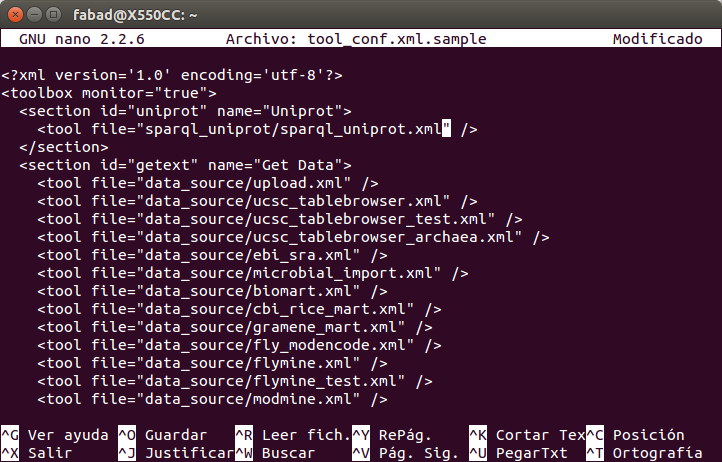
\includegraphics[width=1\textwidth]{figures/register}
\end{figure}

The new tool has been inserted into a new section called Uniprot.

\clearpage

\section{Galaxy Tool Shed}
We have decided to share the new tool we have developed with other Galaxy users through Galaxy Tool Shed. To do this, a repository called \textit{sparql\_uniprot} has been created at \url{https://toolshed.g2.bx.psu.edu/view/fabad/sparql_uniprot}. This repository contains the following files:
\begin{itemize}
	\item \textbf{sparql\_uniprot.py} - The script that query against Uniprot database.
	\item \textbf{sparql\_uniprot.xml} - The configuration file that tells Galaxy how to run sparql\_uniprot.py.
	\item \textbf{tool\_dependencies.xml} - The configuration file that allows Galaxy to manage dependencies.
\end{itemize}

The new file that is not explained before is \textbf{tool\_dependencies.xml} (Appendix 3). It contains information about how galaxy must manage the dependencies that \textbf{sparql\_uniprot.py} has, which are described in \textbf{sparql\_uniprot.xml}. In this case, python module \textit{SPARQLWrapper} is required to run the tool, so \textbf{tool\_dependencies.xml} indicate how to install it. By doing this, when a user download the tool via Galaxy Tool Shed, \textit{SPARQLWrapper} will be downloaded automatically.

Notice that \textit{setup\_virtualenv} action will install python module \textit{SPARQLWrapper} via pip.

\clearpage

\section{Some examples}

Different searches have been made to check if the tool is working correctly. This queries are summarized by the following points: 
\begin{itemize}
	\item Q13563, uniprot identifier, is used to find out different parameters related with it (Figure \ref{fig:example_1a}). 
	\item \textasciicircum and \$ have been used to perform a perfect match search about INS gene (Figure \ref{fig:example_2a}). 
	\item Search about the PTEN gene in the 'sapiens' organism (Figure \ref{fig:example_3a}). 
	\item Search of proteins belong to 'Mouse' organism and It are secreted (Figure \ref{fig:example_4a}).
	\item 'Associates with actin filament appendages that are formed in the inclusion appendages of the parasitophorous vacuole during infection of the host erythrocyte' has been used as function annotation for searching the protein that accomplish it(Figure \ref{fig:example_5a}). 
\end{itemize}

\begin{figure}[h]
	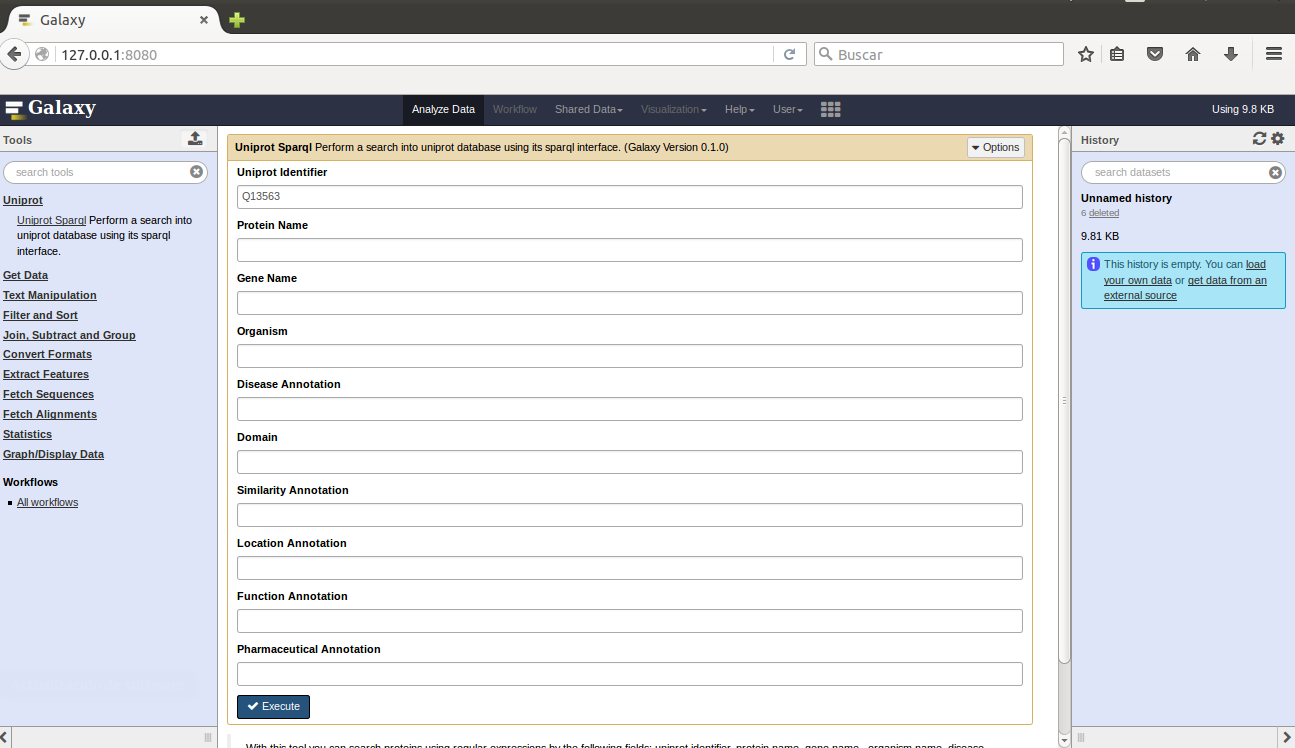
\includegraphics[width=0.9\textwidth]{figures/1a}
	\caption{Search 1}
	\label{fig:example_1a}
\end{figure}
\begin{figure}[h]
	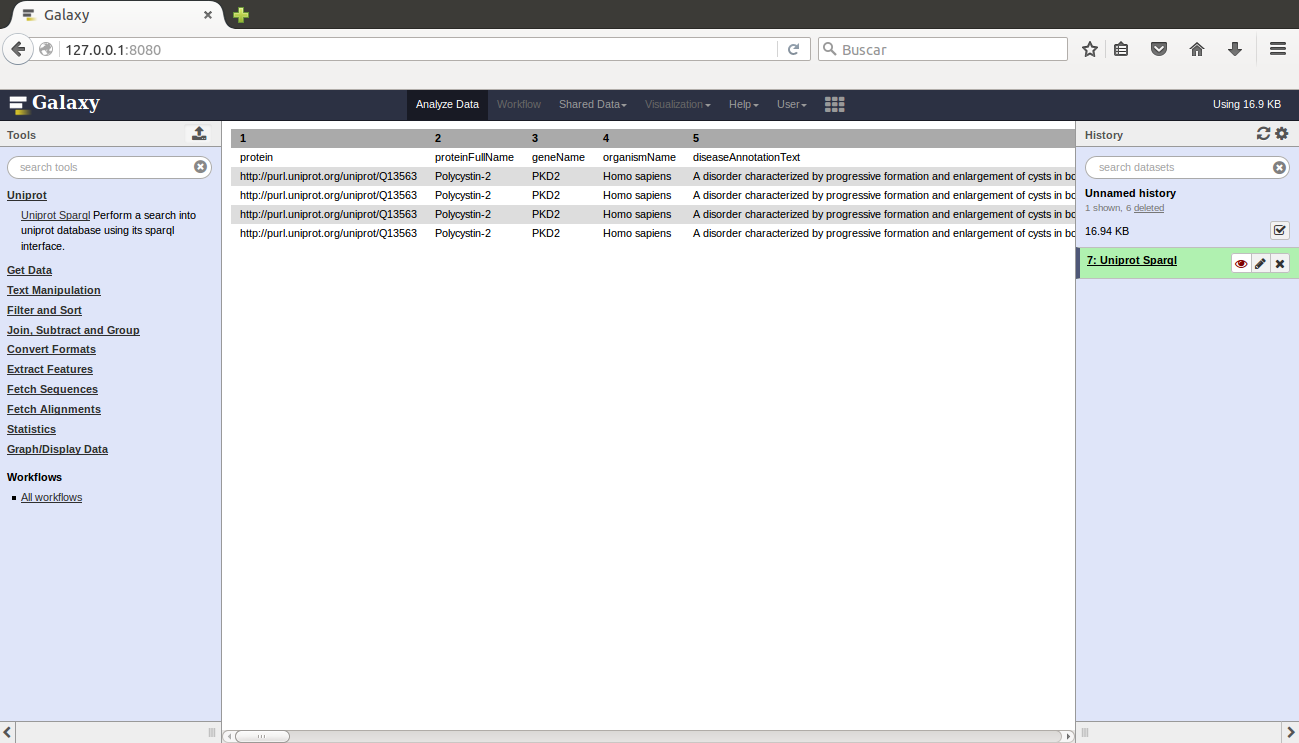
\includegraphics[width=0.9\textwidth]{figures/1b}
	\caption{Results of search 1}
	\label{fig:example_1b}
\end{figure}

\begin{figure}[h]
	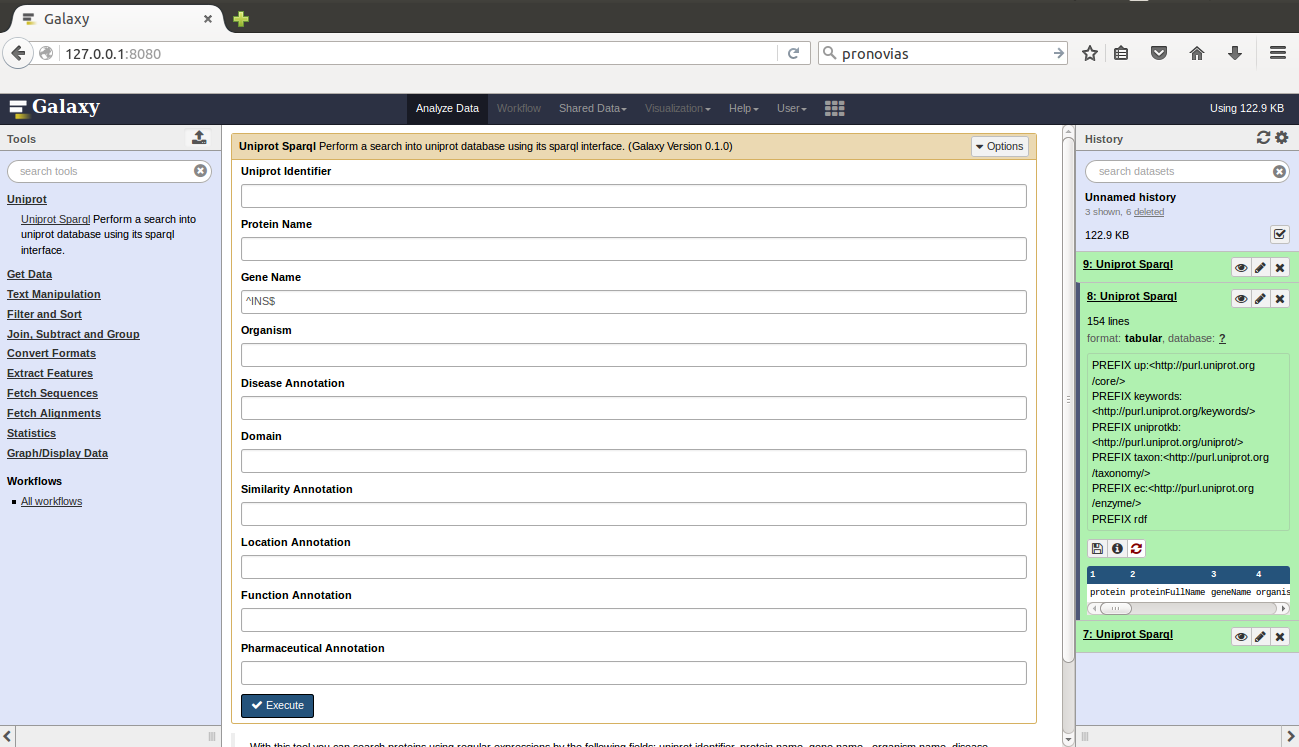
\includegraphics[width=0.9\textwidth]{figures/2a}
	\caption{Search 2}
	\label{fig:example_2a}
\end{figure}
\begin{figure}[h]
	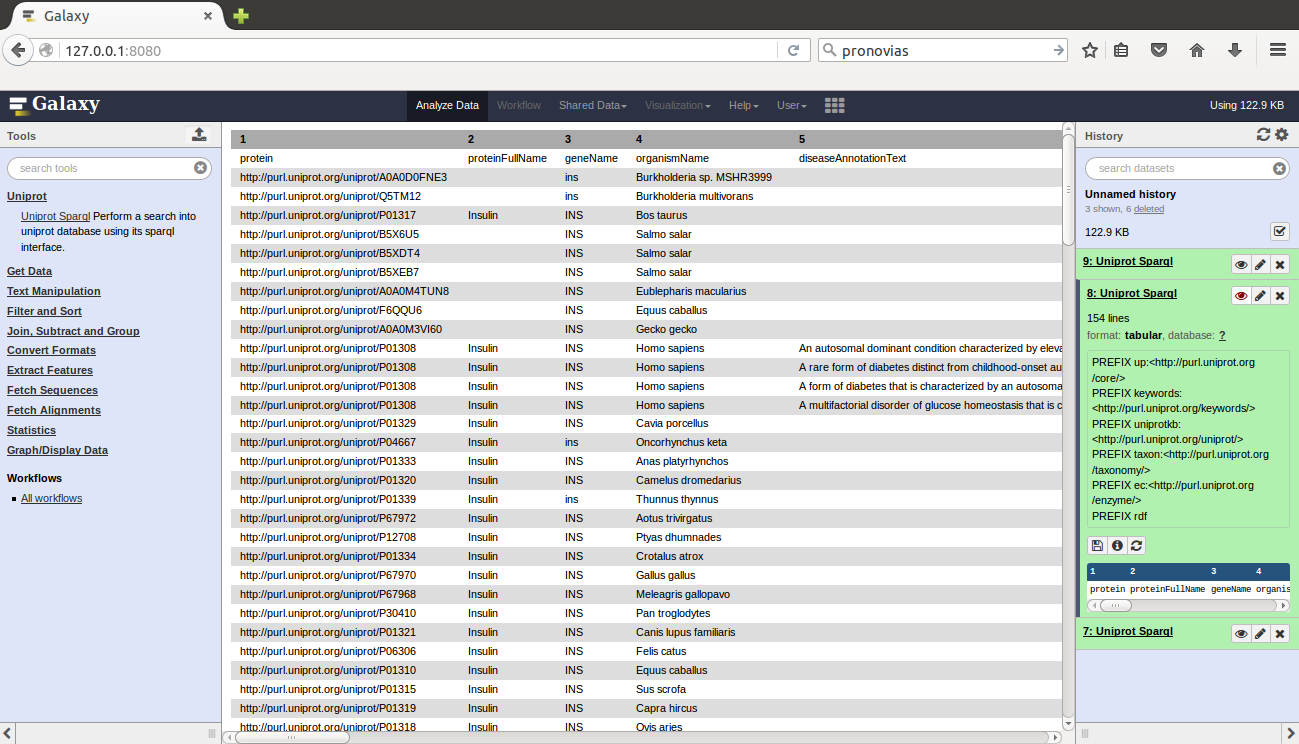
\includegraphics[width=0.9\textwidth]{figures/2b}
	\caption{Results of search 2}
	\label{fig:example_2b}
\end{figure}

\begin{figure}[h]
	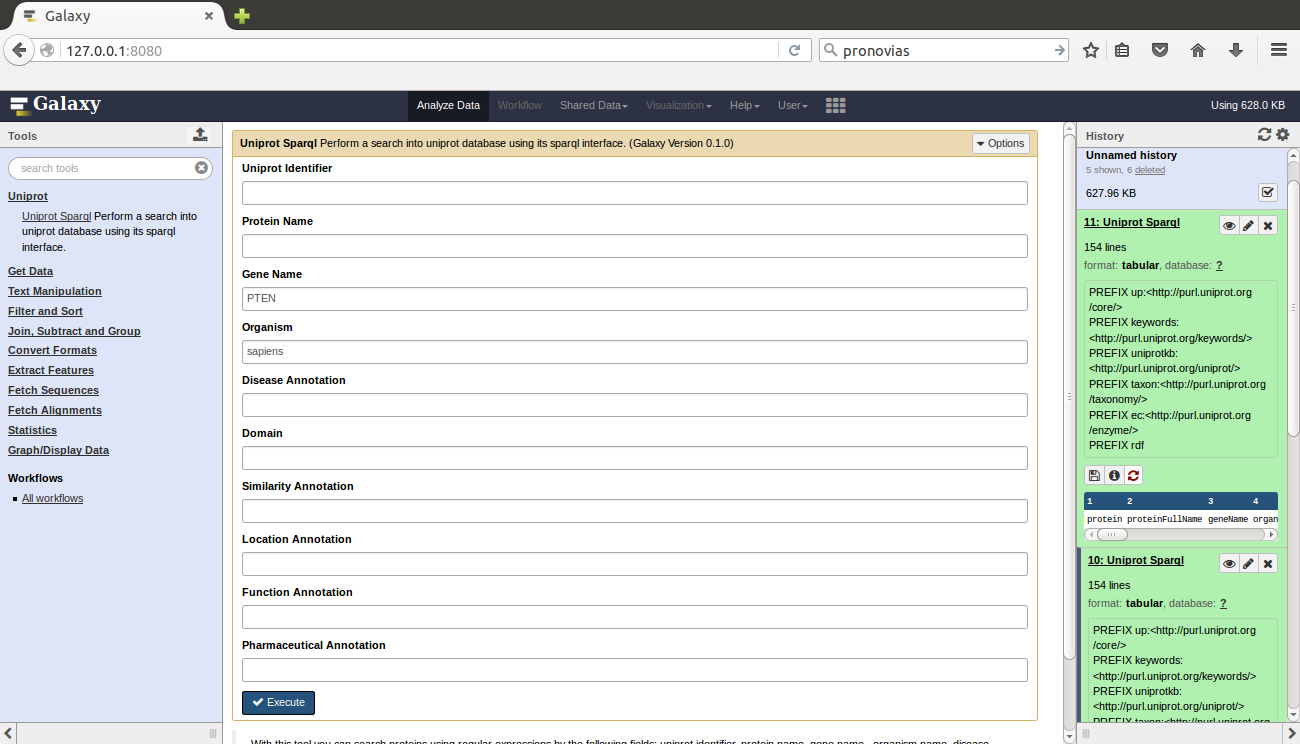
\includegraphics[width=0.9\textwidth]{figures/3a}
	\caption{Search 3}
	\label{fig:example_3a}
\end{figure}
\begin{figure}[h]
	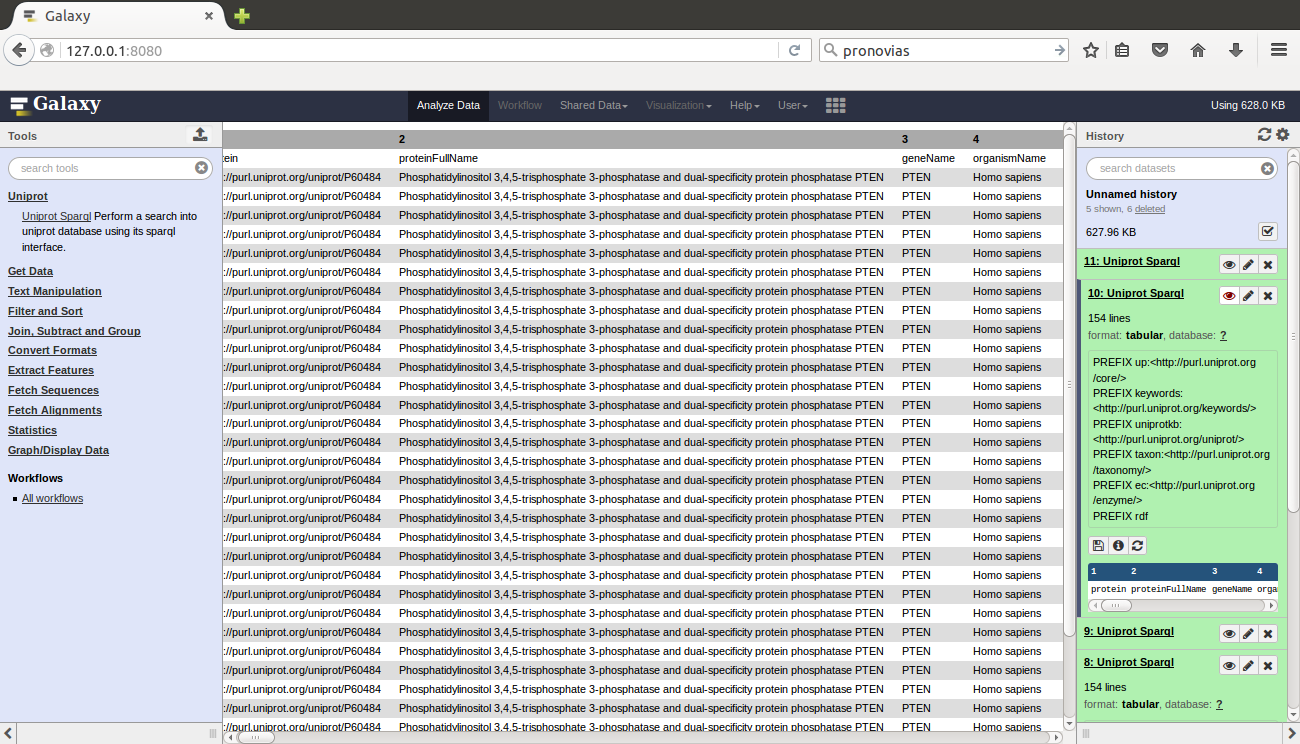
\includegraphics[width=0.9\textwidth]{figures/3b}
	\caption{Results of search 3}
	\label{fig:example_3b}
\end{figure}

\begin{figure}[h]
	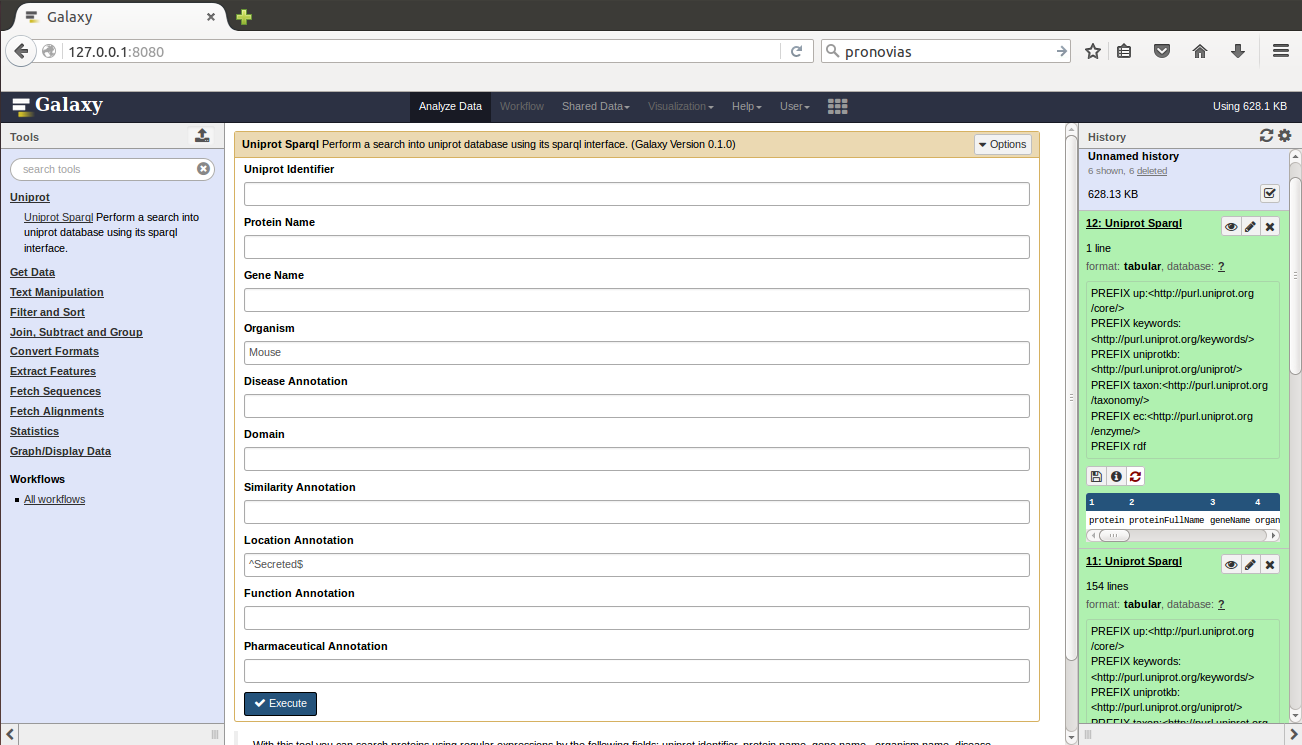
\includegraphics[width=0.9\textwidth]{figures/4a}
	\caption{Search 4}
	\label{fig:example_4a}
\end{figure}
\begin{figure}[h]
	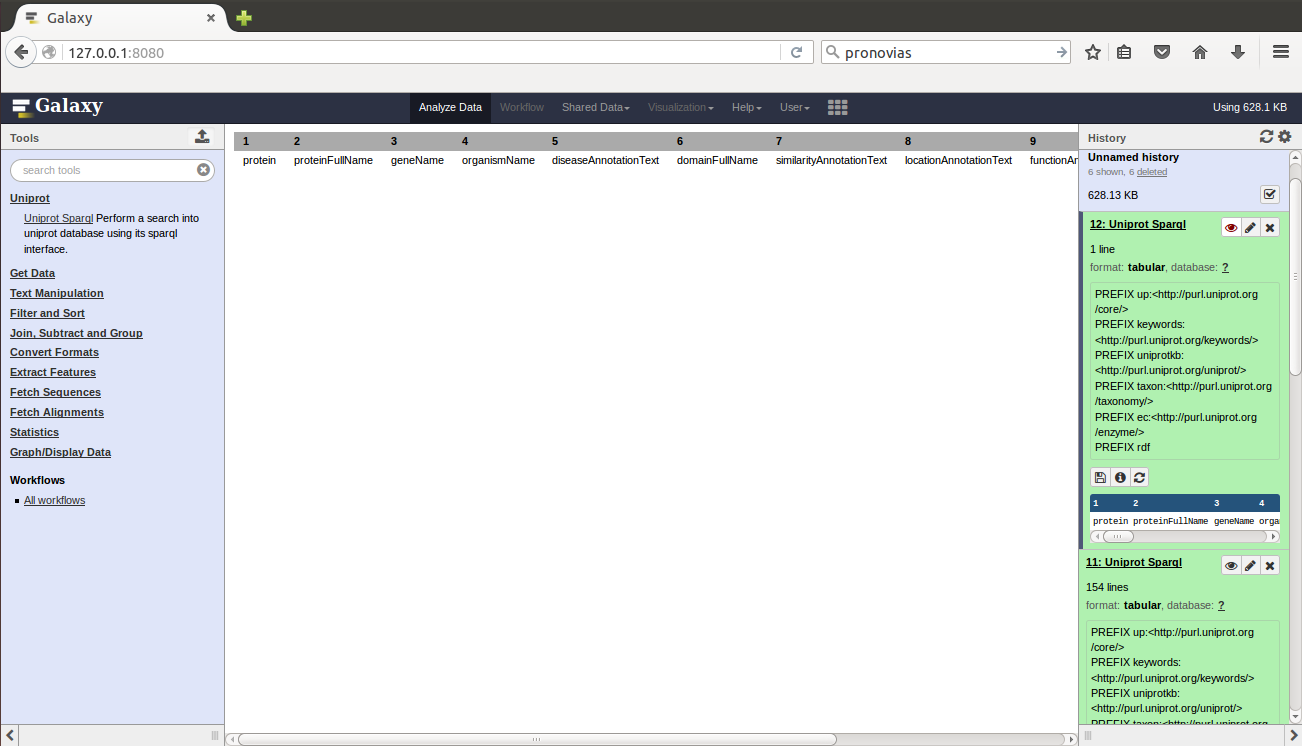
\includegraphics[width=0.9\textwidth]{figures/4b}
	\caption{Results of search 4}
	\label{fig:example_4b}
\end{figure}


\begin{figure}[h]
	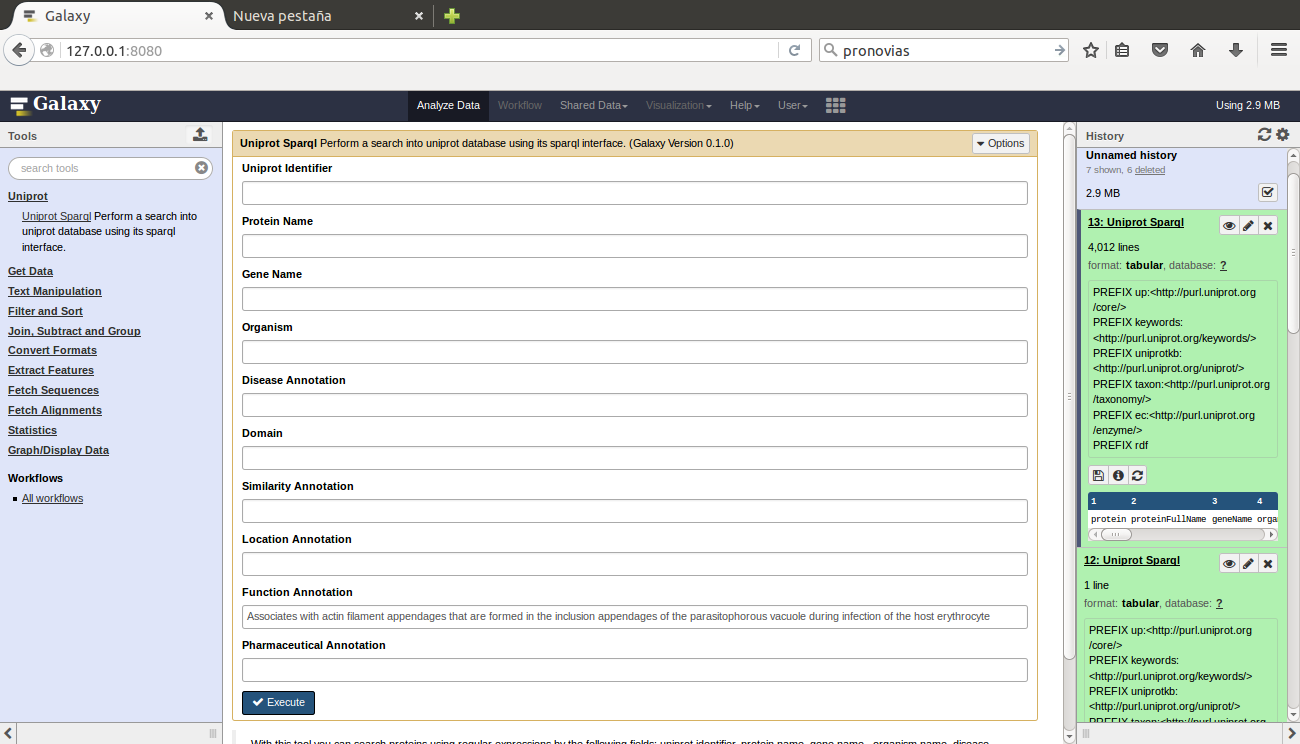
\includegraphics[width=0.9\textwidth]{figures/5a}
	\caption{Search 5}
	\label{fig:example_5a}
\end{figure}
\begin{figure}[h]
	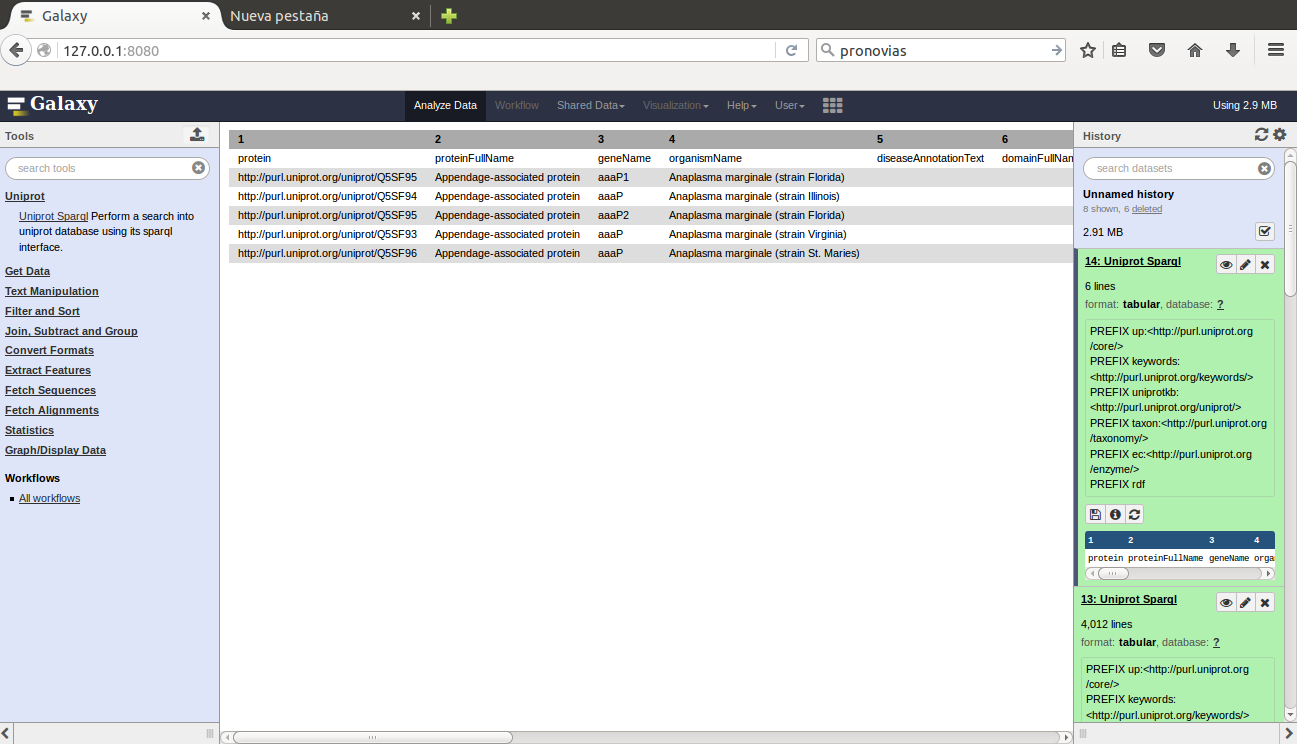
\includegraphics[width=0.9\textwidth]{figures/5b}
	\caption{Results of search 5}
	\label{fig:example_5b}
\end{figure}

\clearpage


\section*{Appendix 1}
\begin{Verbatim}
from SPARQLWrapper import SPARQLWrapper, JSON
import sys

# Constante con los prefijos comunes a usar en queries
COMMON_PREFIXES = """
        PREFIX up:<http://purl.uniprot.org/core/>
        PREFIX keywords:<http://purl.uniprot.org/keywords/>
        PREFIX uniprotkb:<http://purl.uniprot.org/uniprot/>
        PREFIX taxon:<http://purl.uniprot.org/taxonomy/>
        PREFIX ec:<http://purl.uniprot.org/enzyme/>
        PREFIX rdf:<http://www.w3.org/1999/02/22-rdf-syntax-ns#>
        PREFIX rdfs:<http://www.w3.org/2000/01/rdf-schema#>
        PREFIX skos:<http://www.w3.org/2004/02/skos/core#>
        PREFIX owl:<http://www.w3.org/2002/07/owl#>
        PREFIX bibo:<http://purl.org/ontology/bibo/>
        PREFIX dc:<http://purl.org/dc/terms/>
        PREFIX xsd:<http://www.w3.org/2001/XMLSchema#>
        PREFIX faldo:<http://biohackathon.org/resource/faldo#>
"""

# Lista con los nombres de las variables que obtenemos de la base de datos.
paramList = [
    'protein',
    'proteinFullName',
    'geneName',
    'organismName',
    'diseaseAnnotationText',
    'domainFullName',
    'similarityAnnotationText',
    'locationAnnotationText',
    'functionAnnotationText',
    'pharmaceuticalAnnotationText']


def buildQuery(
        proteinId,
        proteinName,
        geneName,
        organismName,
        diseaseAnnotation,
        domainName,
        similarityAnnotation,
        locationAnnotation,
        functionAnnotation,
        pharmaceuticalAnnotation):
    query = COMMON_PREFIXES
    query += "select distinct \n"
    query += "      ?protein\n"
    query += "      ?proteinFullName\n"
    query += "      ?geneName\n"
    query += "      ?organismName\n"
    query += "      ?diseaseAnnotationText\n"
    query += "      ?domainFullName\n"
    query += "      ?similarityAnnotationText\n"
    query += "      ?locationAnnotationText\n"
    query += "      ?functionAnnotationText\n"
    query += "      ?pharmaceuticalAnnotationText\n"
    query += "where{\n"

    query += "      ?protein a up:Protein .\n"

    if (proteinId != ''):
        query += "      VALUES ?protein {uniprotkb:" + proteinId + "}\n"

    query += "\n"

    if (proteinName == ''):
        query += "      OPTIONAL {\n"
    query += "      ?protein up:recommendedName ?proteinName .\n"
    query += "      ?proteinName up:fullName ?proteinFullName . \n"
    if (proteinName != ''):
        query += "      filter( regex(str(?proteinFullName), " + \
            '"' + proteinName + '"' + ",\"i\" )) .\n"
    if (proteinName == ''):
        query += "      }\n"
    query += "\n"

    if (geneName == ''):
        query += "      OPTIONAL {\n"
    query += "      ?protein up:encodedBy ?gene .\n"
    query += "      ?gene skos:prefLabel ?geneName .\n"
    if (geneName != ''):
        query += "      filter( regex(str(?geneName), " + \
            '"' + geneName + '"' + ",\"i\" )) .\n"
    if (geneName == ''):
        query += "      }\n"

    query += "\n"

    if (organismName == ''):
        query += "      OPTIONAL {\n"
    query += "      ?protein up:organism ?organism .\n"
    query += "      ?organism up:scientificName ?organismName .\n"
    if (organismName != ''):
        query += "      filter( regex(str(?organismName), " + \
            '"' + organismName + '"' + ",\"i\" )) .\n"
    if (organismName == ''):
        query += "      }\n"

    query += "\n"

    if (diseaseAnnotation == ''):
        query += "      OPTIONAL {\n"
    query += "      ?protein up:annotation ?diseaseAnnotation .\n"
    query += "      ?diseaseAnnotation a up:Disease_Annotation .\n"
    query += "      ?diseaseAnnotation up:disease ?disease .\n"
    query += "      ?disease rdfs:comment ?diseaseAnnotationText\n"
    if (diseaseAnnotation != ''):
        query += "      filter( regex(str(?diseaseAnnotationText), " + \
            '"' + diseaseAnnotation + '"' + ",\"i\" )) .\n"
    if (diseaseAnnotation == ''):
        query += "      }\n"

    query += "\n"

    if (domainName == ''):
        query += "      OPTIONAL {\n"
    query += "      ?protein up:domain ?domain .\n"
    query += "      ?domain up:recommendedName ?domainName .\n"
    query += "      ?domainName up:fullName ?domainFullName .\n"
    if (domainName != ''):
        query += "      filter( regex(str(?domainFullName), " + \
            '"' + domainName + '"' + ",\"i\" )) .\n"
    if (domainName == ''):
        query += "      }\n"

    query += "\n"

    if (similarityAnnotation == ''):
        query += "      OPTIONAL {\n"
    query += "      ?protein up:annotation ?similarityAnnotation .\n"
    query += "      ?similarityAnnotation a up:Similarity_Annotation .\n"
    query += "      ?similarityAnnotation rdfs:comment ?similarityAnnotationText .\n"
    if (similarityAnnotation != ''):
        query += "      filter( regex(str(?similarityAnotationText), " + \
            '"' + similarityAnnotation + '"' + ",\"i\" )) .\n"
    if (similarityAnnotation == ''):
        query += "      }\n"

    query += "\n"

    if (locationAnnotation == ''):
        query += "      OPTIONAL {\n"
    query += "      ?protein up:annotation ?locationAnnotation .\n"
    query += "      ?locationAnnotation a up:Subcellular_Location_Annotation .\n"
    query += "      ?locationAnnotation up:locatedIn ?location .\n"
    query += "      ?location up:cellularComponent ?cellComponent .\n"
    query += "      ?cellComponent rdfs:comment ?locationAnnotationText .\n"
    if (locationAnnotation != ''):
        query += "      filter( regex(str(?locationAnnotationText), " + \
            '"' + locationAnnotation + '"' + ",\"i\" )) .\n"
    if (locationAnnotation == ''):
        query += "      }\n"

    query += "\n"

    if (functionAnnotation == ''):
        query += "      OPTIONAL {\n"
    query += "      ?protein up:annotation ?functionAnnotation .\n"
    query += "      ?functionAnnotation a up:Function_Annotation .\n"
    query += "      ?functionAnnotation rdfs:comment ?functionAnnotationText .\n"
    if (functionAnnotation != ''):
        query += "      filter( regex(str(?functionAnnotationText), " + \
            '"' + functionAnnotation + '"' + ",\"i\" )) .\n"
    if(functionAnnotation == ''):
        query += "      }\n"

    query += "\n"

    if (pharmaceuticalAnnotation == ''):
        query += "      OPTIONAL {\n"
    query += "      ?protein up:annotation ?pharmaceuticalAnnotation .\n"
    query += "      ?pharmaceuticalAnnotation a up:Pharmaceutical_Annotation .\n"
    query += "      ?pharmaceuticalAnnotation rdfs:comment ?pharmaceuticalAnnotationText .\n"
    if (pharmaceuticalAnnotation != ''):
        query += "      filter( regex(str(?pharmaceuticalAnnotationText), " + \
            '"' + pharmaceuticalAnnotation + '"' + ",\"i\" )) .\n"
    if (pharmaceuticalAnnotation == ''):
        query += "      }\n"
    query += "}\n"
    #query += "limit 30\n"

    return query


def printResults(json, output):
    # Abrir fichero para escritura
    fileRes = open(output, 'w')
    # Imprimir cabecera
    for param in paramList:
        fileRes.write(param + "\t")
    fileRes.write("\n")

    # El formato json se puede recorrer de esta manera
    # para ir obteniendo valores de la respuesta.
    for entrada in json["results"]["bindings"]:
        for param in paramList:
            if (entrada.get(param)):
                fileRes.write(entrada.get(param)["value"] + "\t")
            else:
                fileRes.write("\t")
        fileRes.write("\n")
    fileRes.close()


def sparqlwrap(
        proteinId,
        proteinName,
        geneName,
        organismName,
        diseaseAnnotation,
        domainName,
        similarityAnnotation,
        locationAnnotation,
        functionAnnotation,
        pharmaceuticalAnnotation,
        output):

    query = buildQuery(
        proteinId,
        proteinName,
        geneName,
        organismName,
        diseaseAnnotation,
        domainName,
        similarityAnnotation,
        locationAnnotation,
        functionAnnotation,
        pharmaceuticalAnnotation)
    print query

    # Creamos un objeto del tipo SPARQLWrapper indicando en que
    # direccion esta el servicio que recibe consultas en sparql
    # y responde a estas.
    sparql = SPARQLWrapper('http://sparql.uniprot.org/sparql')

    # Especificamos la consulta que queremos hacer en sparql.
    sparql.setQuery(query)

    # Indicamos en que formato queremos que nos devuelva
    # los resultados de la consulta. Puede ser json, xml,
    # rfd, turtle... Simplemente son distintos formatos
    # para representar los datos en ficheros de texto.
    sparql.setReturnFormat(JSON)

    # Esta es la instruccion que realiza la consulta a
    # uniprot. Devuelve un objeto de python que hay que
    # tratar.
    print "Ejecutando query"
    results = sparql.query()

    # Con esto, convertimos el objeto devuelto por
    # el servicio al formato que especificamos antes.
    # En este caso, json.
    print "Conviertiendo a json"
    json = results.convert()
    print "Fin conversion a json"

    # Dentro de la variable results tenemos informacion
    # (metadatos) de lo que ha devuelto el servidor de
    # uniprot.
    print results.info()

    # Imprimir resultados
    printResults(json, output)


# Obtener parametros de la linea de comandos.
proteinId = sys.argv[1]
proteinName = sys.argv[2]
geneName = sys.argv[3]
organismName = sys.argv[4]
diseaseAnnotation = sys.argv[5]
domainName = sys.argv[6]
similarityAnnotation = sys.argv[7]
locationAnnotation = sys.argv[8]
functionAnnotation = sys.argv[9]
pharmaceuticalAnnotation = sys.argv[10]
output = sys.argv[11]

# Llamada a la funcion que realiza la consulta.
sparqlwrap(
    proteinId,
    proteinName,
    geneName,
    organismName,
    diseaseAnnotation,
    domainName,
    similarityAnnotation,
    locationAnnotation,
    functionAnnotation,
    pharmaceuticalAnnotation,
    output)
\end{Verbatim}

\pagebreak
\section*{Appendix 2}
\begin{Verbatim}
<tool id="sparql_uniprot" name="Uniprot Sparql" version="0.1.0">
  <description>Perform a search into uniprot database using its sparql interface.</description>
  <requirements>
    <requirement type="binary">python</requirement>
    <requirement type="package" version="1.7.6">SPARQLWrapper</requirement>
  </requirements>
  <command interpreter="python">
    sparql_uniprot.py "${protein}" "${proteinName}"
    "${geneName}" "${organismName}"
    "${diseaseAnnotation}" "${domainName}"
    "${similarityAnnotation}" "${locationAnnotation}"
    "${functionAnnotation}" "${pharmaceuticalAnnotation}"
    "${output}"
  </command>
  <inputs>
    <param name="protein" type="text" label="Uniprot Identifier"/>

    <param name="proteinName" type="text" label="Protein Name">
	<!-- sanitizer para que nos deje usar el caracter $ -->
	<sanitizer sanitize="False"/>
    </param>

    <param name="geneName" type="text" label="Gene Name">
	<sanitizer sanitize="False"/>
    </param>

    <param name="organismName" type="text" label="Organism">
	<sanitizer sanitize="False"/>
    </param>

    <param name="diseaseAnnotation" type="text" label="Disease Annotation">
	<sanitizer sanitize="False"/>
    </param>

    <param name="domainName" type="text" label="Domain">
	<sanitizer sanitize="False"/>
    </param>

    <param name="similarityAnnotation" type="text" label="Similarity Annotation">
	<sanitizer sanitize="False"/>
    </param>

    <param name="locationAnnotation" type="text" label="Location Annotation">
	<sanitizer sanitize="False"/>
    </param>

    <param name="functionAnnotation" type="text" label="Function Annotation">
	<sanitizer sanitize="False"/>
    </param>

    <param name="pharmaceuticalAnnotation" type="text" label="Pharmaceutical Annotation">
	<sanitizer sanitize="False"/>
    </param>
  </inputs>

  <outputs>
    <data format="tabular" name="output" />
  </outputs>

  <help>
With this tool you can search proteins using regular expressions
by the following fields:uniprot identifier, protein name, gene name,
organism name, disease annotation, domain name,similarity annotation,
location annotation, function annotation or pharmaceutical annotation.
You can fill the fields you want and the tool will return all the data
found in uniprot by filling the other fields. Results will be stored
in a tabular format. If you want to search the exact match of a field
you should use ^parameter$, for example ^insulin$.
  </help>

</tool>
\end{Verbatim}
\pagebreak
\section*{Appendix 3}
\begin{Verbatim}
<?xml version="1.0"?>
<tool_dependency>
  <package name="SPARQLWrapper" version="1.7.6">
    <readme>
      Install SPARQLWrapper via virtualenv.
    </readme>
    <install version="1.0">
      <actions>
        <action type="setup_virtualenv">SPARQLWrapper==1.7.6</action>
      </actions>
    </install>
  </package>
</tool_dependency>
\end{Verbatim}
\end{document}




















